\documentclass[border=10pt]{standalone}

\usepackage{tikz}
\usepackage{tikzsymbols}
\usetikzlibrary{calc,patterns,shapes.geometric}

\def\centerarc[#1](#2)(#3:#4:#5){\draw[#1] ($(#2)+({#5*cos(#3)},{#5*sin(#3)})$) arc (#3:#4:#5);}

\begin{document}
	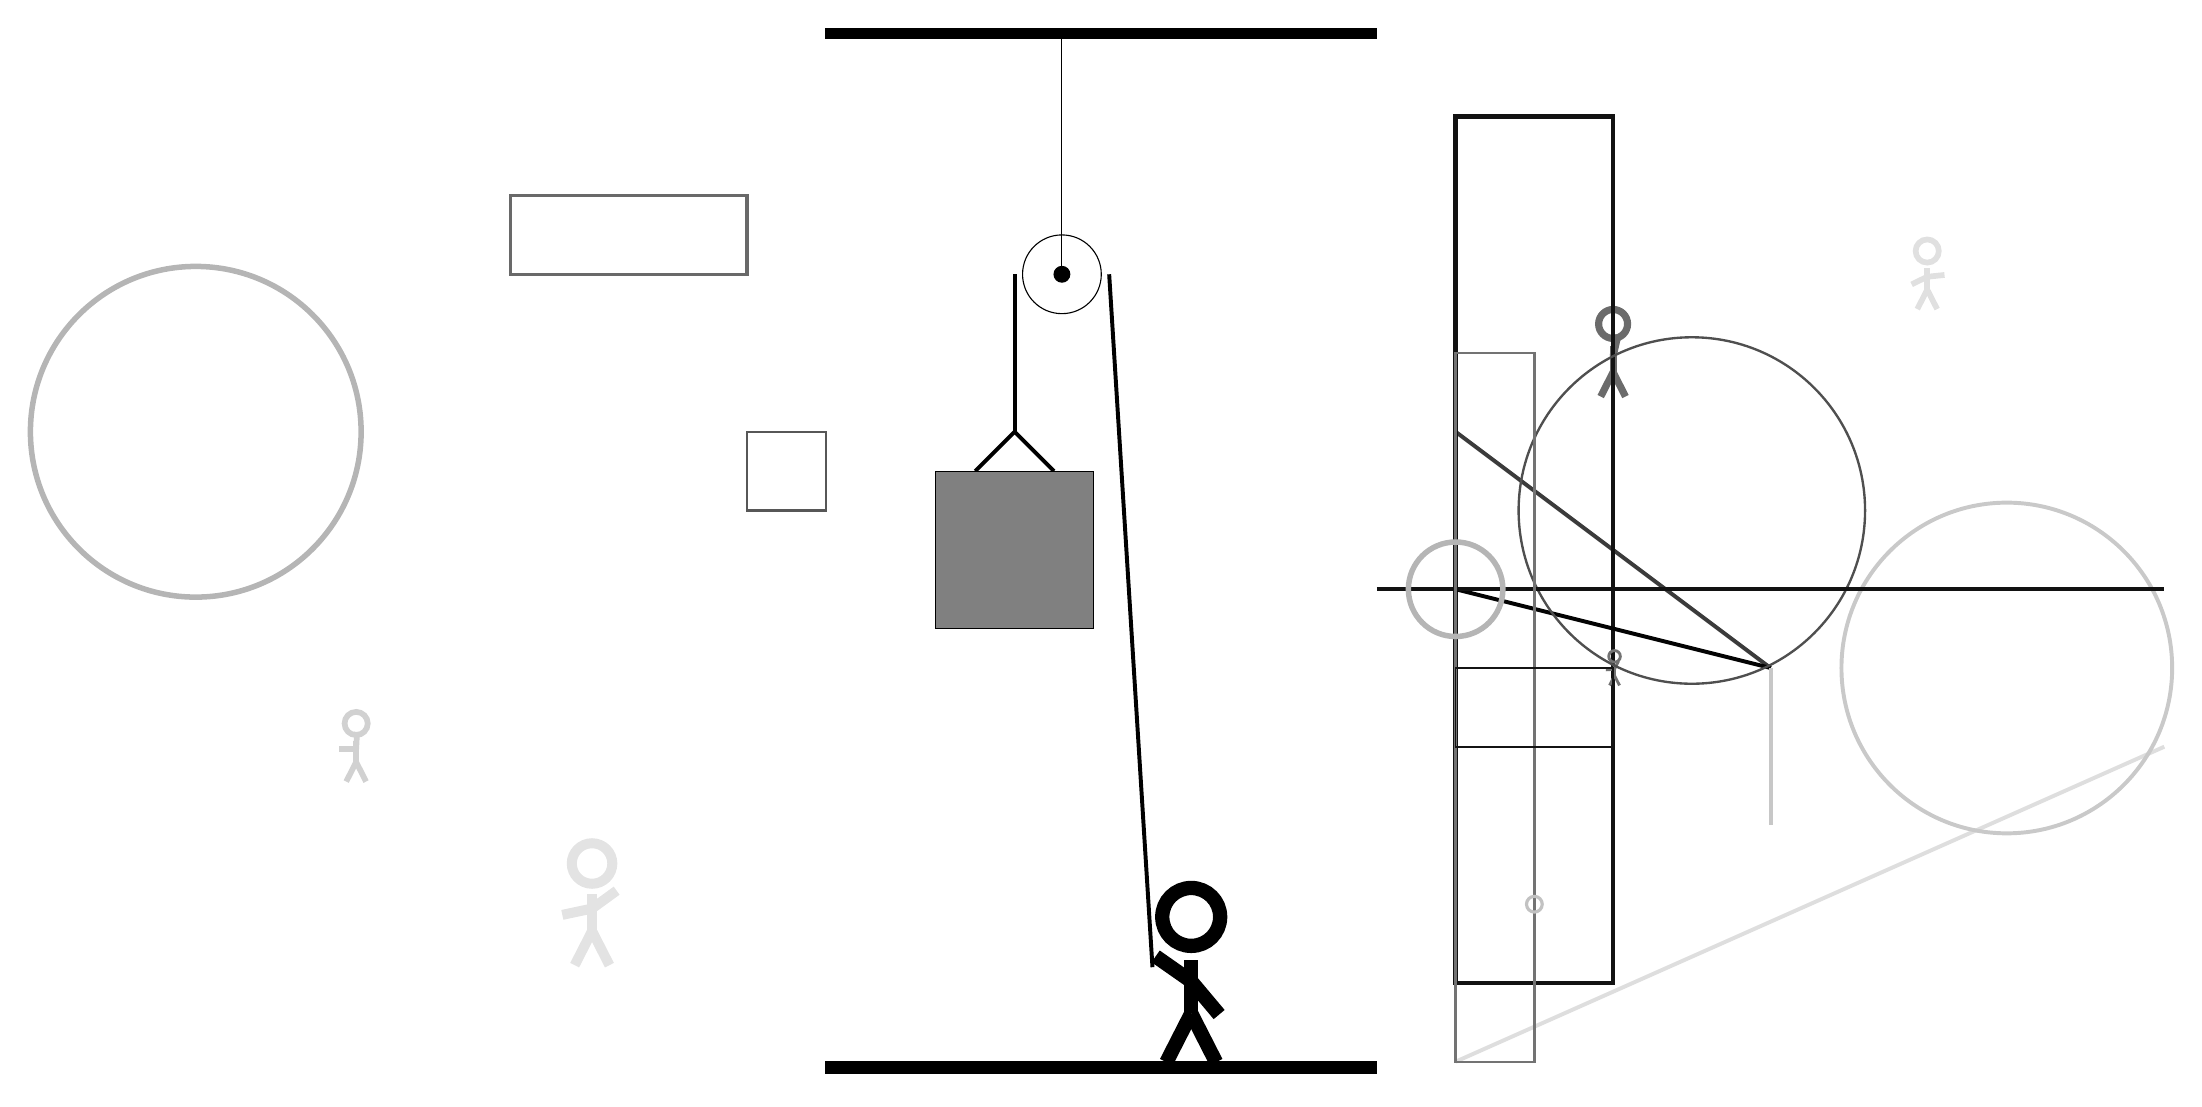
\begin{tikzpicture}
		%%%%% START %%%%%
		
		\draw[fill=black] (-2, 10) rectangle (5, 10.125);
		
		\draw (1, 7) circle (0.5);
		\draw[fill=black] (1, 7) circle (0.1);
		\draw (1, 10) -- (1, 7);
		
		\node[line width=0.7mm, color=black!18] at (-8, 1) {\Strichmaxerl[4][0][87]};
		
		\node[line width=0.6mm, color=black!58] at (8, 6) {\Strichmaxerl[5][90][77]};
		\draw[line width=0.3mm, color=black!66] (-2, 4) rectangle (-3, 5);
		\node[line width=0.2mm, color=black!11] at (-5, -1) {\Strichmaxerl[7][12][36]};
		\draw[line width=0.4mm, color=black!59] (-3, 8) rectangle (-6, 7);
		
		\draw[line width=0.5mm, color=black!77](10, 2) -- (6, 5);
		
		\node[line width=0.5mm, color=black!12] at (12, 7) {\Strichmaxerl[4][26][6]};
		
		\draw[line width=0.5mm, color=black!13](6, -3) -- (15, 1);
		\draw [line width=0.7mm, color=black!29](-10, 5) circle (2.1);
		
		\draw[line width=0.6mm, color=black!93] (6, -2) rectangle (8, 9);
		\draw[line width=0.5mm, color=black!63](-7, -3) -- (-7, -3);
		\node[line width=0.7mm, color=black!55] at (8, 2) {\Strichmaxerl[2][4][64]};
		\draw[line width=0.5mm, color=black!99](10, 2) -- (6, 3);
		
		\draw [line width=0.5mm, color=black!21](13, 2) circle (2.1);
		\draw [line width=0.3mm, color=black!69](9, 4) circle (2.2);
		\draw[line width=0.5mm, color=black!93](5, 3) -- (15, 3);
		
		\draw[line width=0.3mm, color=black!55] (7, 6) rectangle (6, -3);
		\draw[line width=0.5mm, color=black!22](10, 2) -- (10, 0);
		\draw[line width=0.2mm, color=black!92] (6, 1) rectangle (8, 2);
		\draw [line width=0.4mm, color=black!24](7, -1) circle (0.1);
		\draw [line width=0.7mm, color=black!29](6, 3) circle (0.6);
		
		
		\draw[line width=0.5mm] (-0.1, 4.5) -- (0.4, 5.0) -- (0.9, 4.5);
		\draw[fill=black!50] (-0.6, 4.5) rectangle (1.4, 2.5);
		
		\draw[line width=0.5mm] (0.4, 7) -- (0.4, 5.0);
		\centerarc[line width=0.5mm](1, 7)(0:180:0.6);
		\draw[line width=0.5mm](1.6, 7) -- (2.15, -1.8);
		
		\node at (2.6, -1.9) {\Strichmaxerl[10][-35][-50]};
		
		\draw[fill=black] (-2, -3) rectangle (5, -3.15);
		
		%%%%% END %%%%%
	\end{tikzpicture}
\end{document}